\documentclass[11pt]{beamer}
\usetheme{Boadilla}
\usepackage[utf8]{inputenc}
\usepackage{amsmath}
\usepackage{amsfonts}
\usepackage{amssymb}
\usepackage{graphicx}
\author{Rafsun Islam, Jeremias Eppler}
\useinnertheme{circles}
\title{Malware Project}
%\setbeamercovered{transparent} 
%\setbeamertemplate{navigation symbols}{} 
%\logo{} 
\institute{DSU} 
%\date{} 
\subject{Handwritten Malware} 
\begin{document}

\begin{frame}
\titlepage
\end{frame}

\begin{frame}{Basic Idea}
\begin{center}
	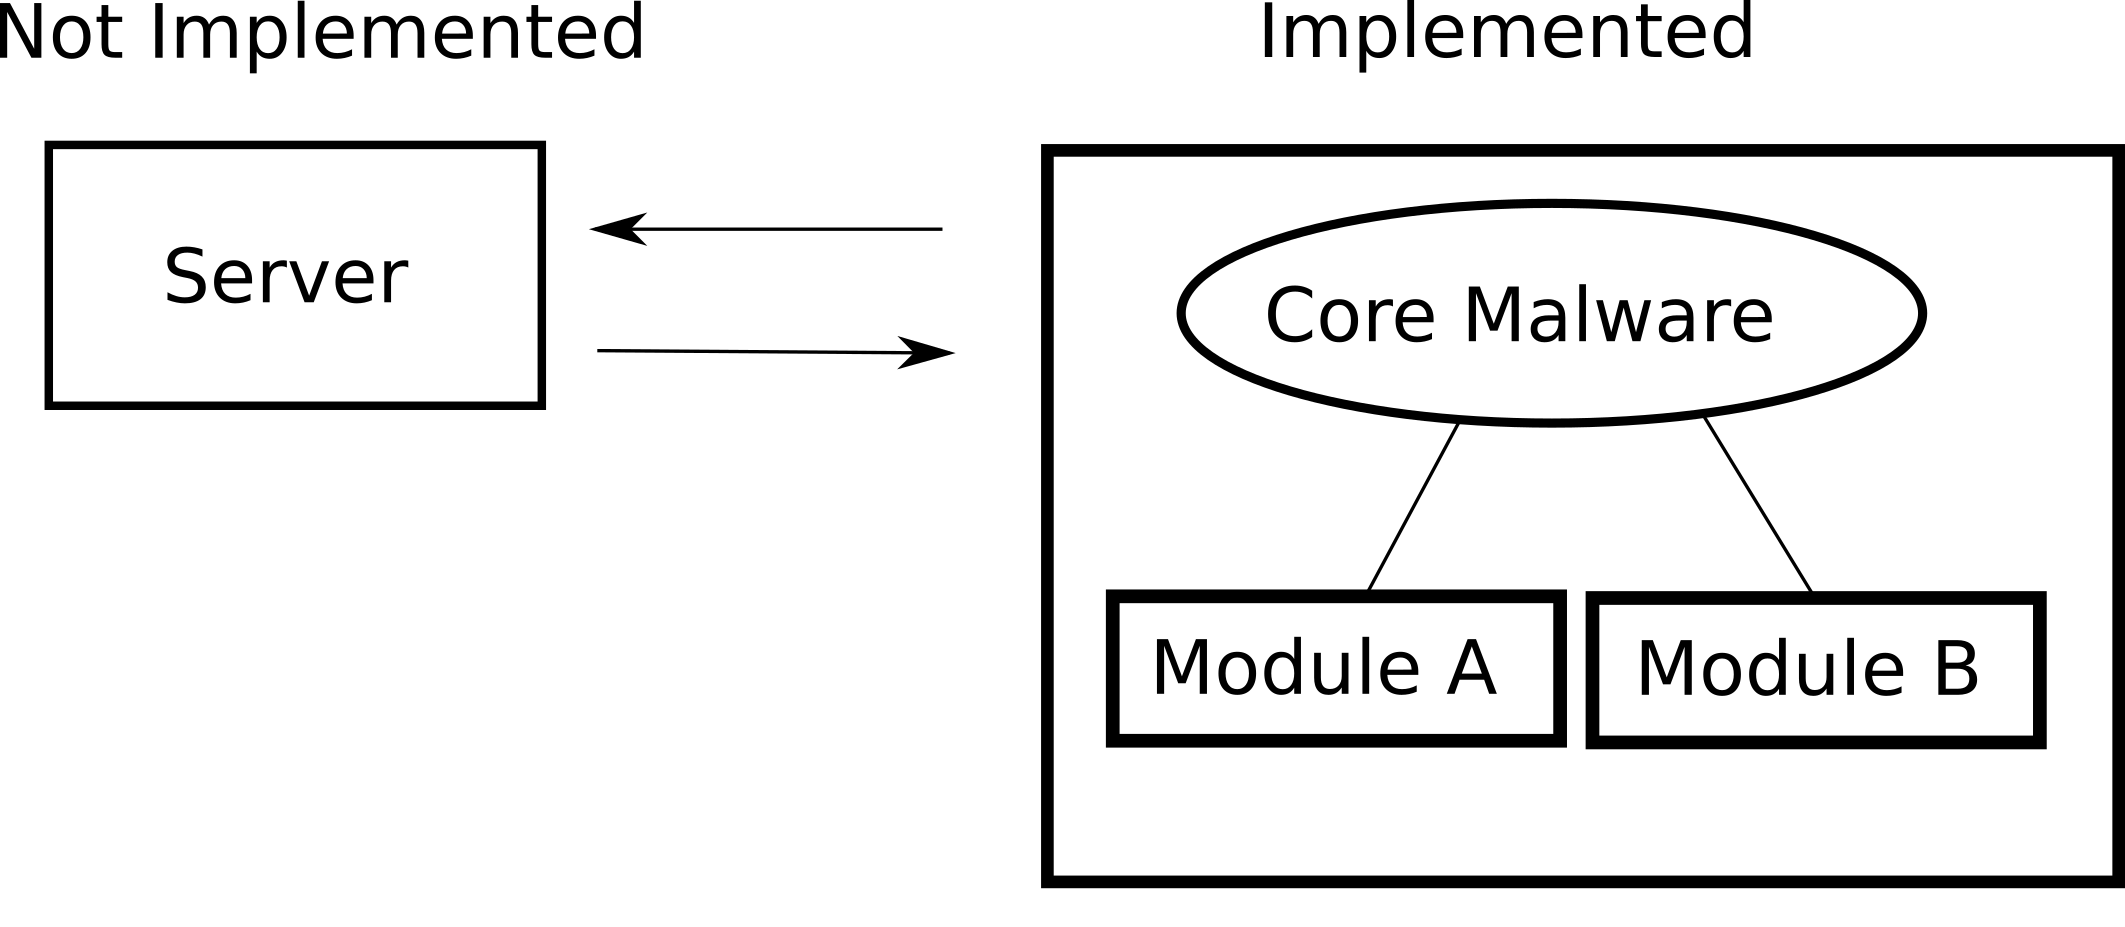
\includegraphics[scale=0.3]{client-server}
\end{center}
\begin{itemize}
	\item basic idea: Malware is modularized
	\item server-agent principle
	\item server controls agent (Core Malware)
	\item agent executes server commands
	\begin{itemize}
		\item start/stop modules
		\item download new modules
		\item uploading information
	\end{itemize}
\end{itemize}
\end{frame}

\begin{frame}{Implemented}
Core Malware features:
\begin{itemize}
	\item executes other modules (Keylogger, ReverseShell)
	\item parses and interprets commands
	\item checks for internet connection
	\item assign it self to to the registry
\end{itemize}
Modules:
\begin{itemize}
	\item PSExecutor - executes PowerShell commands
	\item Keylogger
	\item Reverse Shell (reused)
\end{itemize}
Additional:
\begin{itemize}
	\item Obfuscator
	\item sensless strings/functions (make analysis more difficult)
\end{itemize}
\end{frame}

\end{document}